\section{Peripherals}
\label{sec:periphs}

A simple System on Chip (SoC) including picoVersat, a program and data memory, and the five peripherals
attached to the data bus is shown in Figure~\ref{fig:periphs}.

\begin{figure}[!htbp]
    \centerline{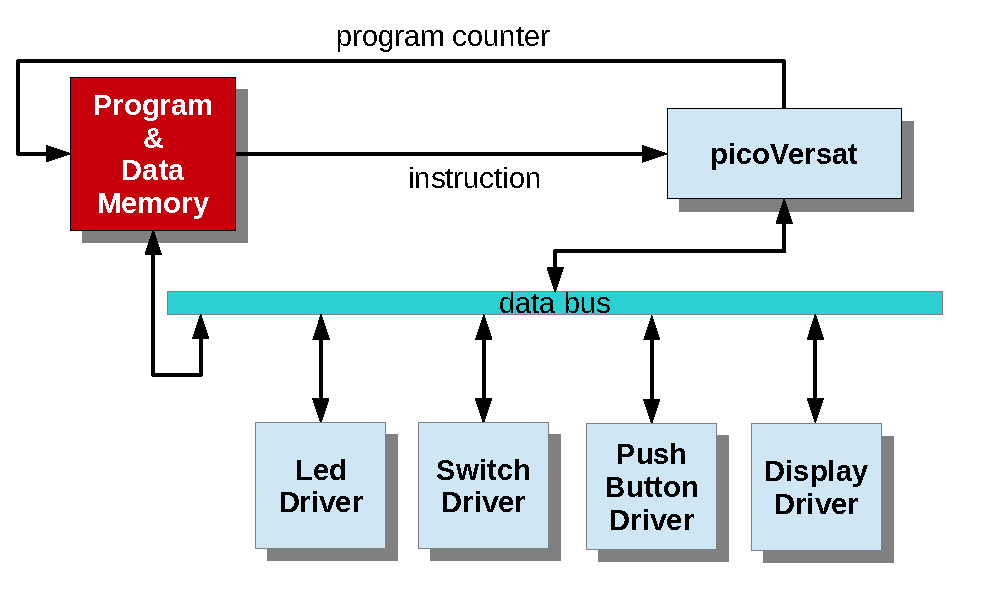
\includegraphics[width=\textwidth]{periphs}}
    \vspace{0cm}\caption{PicoVersat SoC with five peripherals}
    \label{fig:periphs}
\end{figure}

Refer to the memory map in section~\ref{sec:mem_map} to check the base addresses
of the peripherals.

\subsection{PS/2 Driver}
This peripheral can be used to drive a PS/2 interface and using a keyboard to input the data, this driver
makes the management and processing of the incoming data, decoding the pressed key.

\begin{table}[h]
\centering
\begin{tabular}{|l|c|c|l|}
\hline
\multicolumn{1}{|c|}{\bf Name} & {\bf Address} & {\bf Bits} & \multicolumn{1}{c|}{\bf Description} \\ 
\hline \hline
\multicolumn{1}{|l|}{PS2\_BASE} & 610 & 1-0 & PS2 clk and PS2 data.\\ 
\hline
\end{tabular}
\caption{Description of the base address from PS/2 peripheral.}
\label{tab:ps2}
\end{table}

\subsection{Led driver}
This peripheral is a driver to output the value of the LEDs, depending on the value written from the address in the table~\ref{tab:ps2}, the driver decodes which LEDs should be lighted.

\begin{table}[h]
\centering
\begin{tabular}{|l|c|c|l|}
\hline
\multicolumn{1}{|c|}{\bf Name} & {\bf Address} & {\bf Bits} & \multicolumn{1}{c|}{\bf Description} \\ 
\hline \hline
\multicolumn{1}{|l|}{LED\_BASE} & 602 & 3-0 & Each bit corresponds a one LED.\\ 
\hline
\end{tabular}
\caption{Description of the base address from led peripheral.}
\label{tab:led}
\end{table}


\subsection{Switch driver}
This peripheral is a driver for reading the value of the switches, depending on the value read from the address in table~\ref{tab:switch}, the driver saves the status of each switch for PicoVersat use to control the system.

\begin{table}[h]
\centering
\begin{tabular}{|l|c|c|l|}
\hline
\multicolumn{1}{|c|}{\bf Name} & {\bf Address} & {\bf Bits} & \multicolumn{1}{c|}{\bf Description} \\ 
\hline \hline
\multicolumn{1}{|l|}{SWITCH\_BASE} & 604 & 3-0 & Each bit corresponds a one switch.\\ 
\hline
\end{tabular}
\caption{Description of the base address from switch peripheral.}
\label{tab:switch}
\end{table}

\clearpage
\subsection{Push-button driver}
This peripheral drives the value of the buttons and deals with the debounce problem.

\begin{table}[h]
\centering
\begin{tabular}{|l|c|c|l|}
\hline
\multicolumn{1}{|c|}{\bf Name} & {\bf Address} & {\bf Bits} & \multicolumn{1}{c|}{\bf Description} \\ 
\hline \hline
\multicolumn{1}{|l|}{BUTTON\_BASE} & 606 & 1-0  & Reset and start button.\\ 
\hline
\end{tabular}
\caption{Description of the base address from button peripheral.}
\label{tab:button}
\end{table}

\subsection{Display driver}
This peripheral writes to the address from the table~\ref{tab:button}, and the driver decodes which display should be light up, because the data from the 4 displays are connect in parallel and its just necessary to change the value of the anode.

\begin{table}[h]
\centering
\begin{tabular}{|l|c|c|l|}
\hline
\multicolumn{1}{|c|}{\bf Name} & {\bf Address} & {\bf Bits} & \multicolumn{1}{c|}{\bf Description} \\ 
\hline \hline
\multicolumn{1}{|l|}{DISPLAY\_BASE} & 608 & 11-0 & Data bits [7:0] and anode bits [11:8].\\ 
\hline
\end{tabular}
\caption{Description of the base address from display peripheral.}
\label{tab:display}
\end{table}
